\documentclass[aspectratio=169,11pt]{beamer}

\usepackage{fontspec}
\usepackage{polyglossia}
\setmainlanguage{vietnamese}
\setmainfont{Times New Roman}
\setsansfont{Arial}
\usepackage{amsmath,amssymb}
\usepackage{tikz}
\usetikzlibrary{arrows.meta,positioning,shapes.geometric}
\usepackage{graphicx}
\graphicspath{{../images/chapter1/}{../images/chapter2/}{../images/chapter3/}{../images/chapter4/}{../images/chapter6/}{../images/chapter7/}}
\usepackage{booktabs}
\usepackage{array}
\usepackage{ragged2e}
\usepackage{hyperref}

\definecolor{ptitred}{RGB}{145,15,18}
\definecolor{ptitdark}{RGB}{92,92,92}
\definecolor{ptitline}{RGB}{85,45,255}
\definecolor{ptitgray}{RGB}{218,226,218}
\definecolor{softred}{RGB}{252,240,240}

\setbeamertemplate{navigation symbols}{}
\setbeamercolor{normal text}{fg=ptitred,bg=white}
\setbeamercolor{frametitle}{fg=white,bg=ptitred}
\setbeamerfont{frametitle}{series=\bfseries,size=\Large}
\setbeamerfont{title}{series=\bfseries,size=\Large}
\setbeamerfont{subtitle}{series=\bfseries,size=\Large}
\setbeamerfont{author}{size=\small}
\setbeamerfont{institute}{size=\small}

\newcommand{\TopHeader}{%
\begin{tikzpicture}[remember picture,overlay]
  \fill[white] (current page.north west) rectangle ([yshift=-0.90cm]current page.north east);
  \node[anchor=north west,inner sep=0pt] at ([xshift=2.18cm,yshift=-0.10cm]current page.north west) {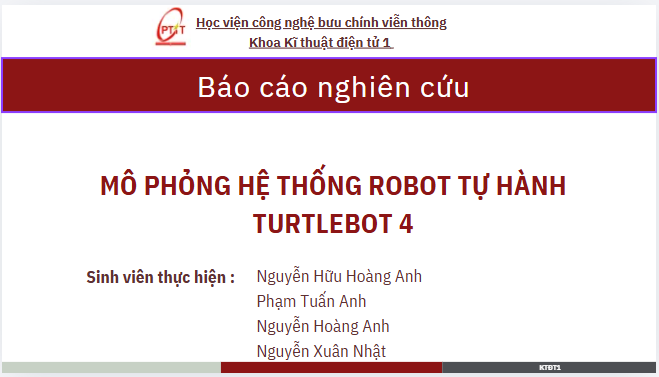
\includegraphics[height=0.54cm]{slide.png}};
  \node[anchor=north,align=center,text=ptitred,font=\bfseries\scriptsize] at ([yshift=-0.14cm]current page.north) {Học viện Công nghệ Bưu chính Viễn thông\\[-1pt]Khoa Kĩ thuật Điện tử 1};
  \fill[ptitred] ([yshift=-0.90cm]current page.north west) rectangle ([yshift=-1.62cm]current page.north east);
  \draw[ptitline,line width=1.1pt] ([yshift=-0.90cm]current page.north west) -- ([yshift=-0.90cm]current page.north east);
  \draw[ptitline,line width=1.1pt] ([yshift=-1.62cm]current page.north west) -- ([yshift=-1.62cm]current page.north east);
\end{tikzpicture}%
}

\newcommand{\BottomFooter}{%
\begin{tikzpicture}[remember picture,overlay]
  \fill[ptitgray] (current page.south west) rectangle ([yshift=0.18cm,xshift=0.34\paperwidth]current page.south west);
  \fill[ptitred] ([xshift=0.34\paperwidth]current page.south west) rectangle ([yshift=0.18cm,xshift=0.68\paperwidth]current page.south west);
  \fill[ptitdark] ([xshift=0.68\paperwidth]current page.south west) rectangle ([yshift=0.18cm]current page.south east);
  \node[anchor=south east,text=white,font=\tiny] at ([xshift=-0.25cm,yshift=0.03cm]current page.south east) {\insertframenumber/\inserttotalframenumber};
\end{tikzpicture}%
}

\setbeamertemplate{frametitle}{%
  \TopHeader
  \vspace*{0.40cm}
  \begin{center}\color{white}\bfseries\Large\insertframetitle\end{center}
  \vspace*{0.48cm}
}
\setbeamertemplate{footline}{\BottomFooter}
\setbeamercolor{block title}{fg=white,bg=ptitred}
\setbeamercolor{block body}{fg=ptitred,bg=softred}
\setbeamerfont{block title}{series=\bfseries}
\setbeamertemplate{itemize item}{\color{ptitred}$\blacktriangleright$}
\setbeamertemplate{itemize subitem}{\color{ptitred}$\circ$}
\newcommand{\img}[2]{\includegraphics[width=#1\linewidth,height=0.48\textheight,keepaspectratio]{#2}}
\newcommand{\topic}[1]{\texttt{#1}}

\title{MÔ PHỎNG ROBOT TỰ HÀNH TURTLEBOT4 LITE}
\subtitle{Tuần tra -- Phát hiện -- Tiếp cận mục tiêu}
\author{Nguyễn Hữu Hoàng Anh \and Phạm Tuấn Anh \and Nguyễn Hoàng Anh \and Nguyễn Xuân Nhật}
\institute{Học viện Công nghệ Bưu chính Viễn thông\\Khoa Kĩ thuật Điện tử 1}
\date{Hà Nội, tháng 06 năm 2026}

\begin{document}

% 1
{\setbeamertemplate{footline}{\BottomFooter}
\begin{frame}[plain]
\TopHeader
\begin{tikzpicture}[remember picture,overlay]
  \node[anchor=north,text=white,font=\bfseries\Large] at ([yshift=-1.03cm]current page.north) {Báo cáo đề tài};
\end{tikzpicture}
\vspace*{1.75cm}
\begin{center}
  {\color{ptitred}\bfseries\LARGE MÔ PHỎNG ROBOT TỰ HÀNH\\[0.12cm]TURTLEBOT4 LITE TRÊN ROS2}
\end{center}
\vspace{0.18cm}
\begin{columns}[c]
\column{0.48\textwidth}
\begin{tabular}{>{\bfseries}r l}
Nhóm thực hiện: & Nguyễn Hữu Hoàng Anh\\
                & Phạm Tuấn Anh\\
                & Nguyễn Hoàng Anh\\
                & Nguyễn Xuân Nhật\\[0.10cm]
GVHD: & TS. Phạm Hoàng Anh
\end{tabular}
\column{0.42\textwidth}
\centering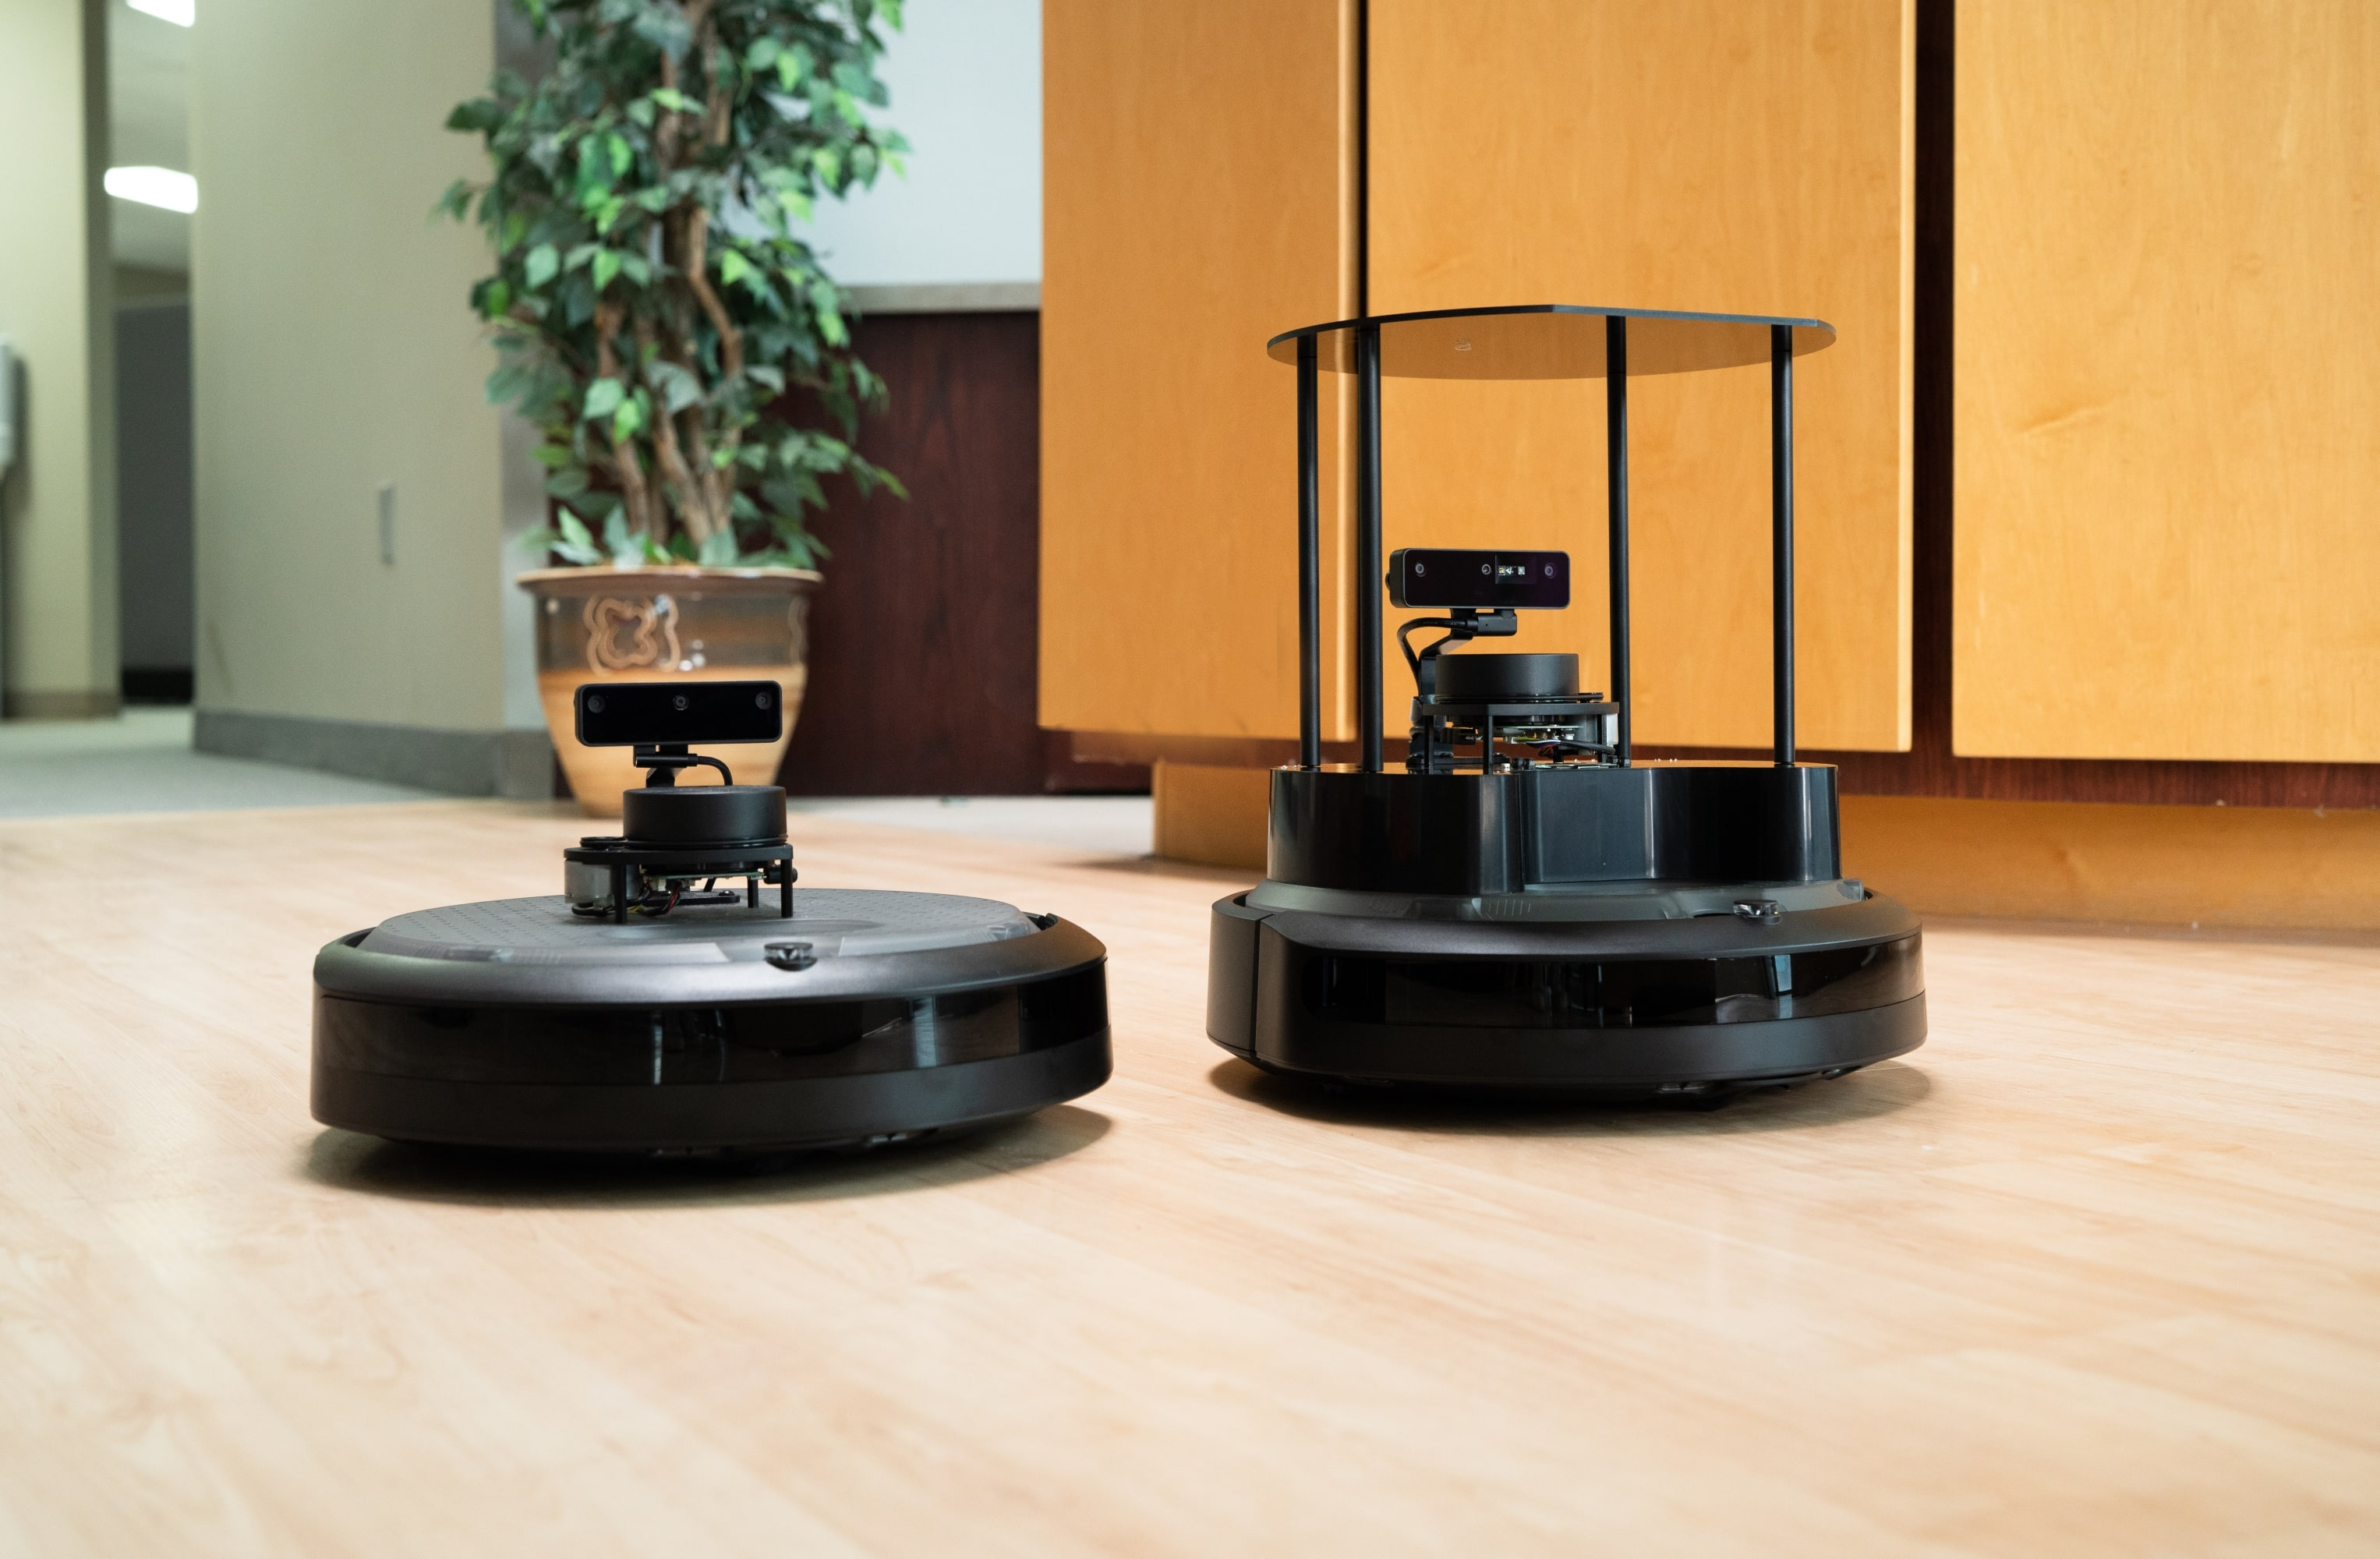
\includegraphics[width=0.75\linewidth,height=0.32\textheight,keepaspectratio]{turtlebot4_lite.png}
\end{columns}
\end{frame}}

% 2
\begin{frame}{Bối cảnh ứng dụng}
\begin{columns}[c]
\column{0.52\textwidth}
\begin{itemize}
  \item Kho vận: tự di chuyển, kiểm kê, vận chuyển hàng nhỏ.
  \item Giám sát: tuần tra khu vực, phát hiện bất thường.
  \item Dịch vụ: dẫn đường, giao nhận trong tòa nhà.
  \item Nhu cầu chung: robot tự định vị, tránh vật cản, phản ứng theo mục tiêu.
\end{itemize}
\column{0.42\textwidth}\centering\img{1.0}{turtlebot4_gazebo.png}
\end{columns}
\end{frame}

% 3
\begin{frame}{Lý do chọn TurtleBot4 Lite + ROS2}
\begin{columns}[c]
\column{0.55\textwidth}
\begin{itemize}
  \item Nền tảng robot giáo dục--nghiên cứu phổ biến.
  \item Hỗ trợ ROS2, Nav2, SLAM Toolbox, Gazebo/Ignition.
  \item Cấu hình vi sai đơn giản, dễ mô phỏng và triển khai thật.
  \item Có LiDAR, camera RGB-D, odometry, TF đầy đủ cho bài toán tự hành.
\end{itemize}
\column{0.38\textwidth}\centering\img{1.0}{turtlebot4_lite.png}
\end{columns}
\end{frame}

% 4
\begin{frame}{Bài toán nghiên cứu}
\begin{block}{Nhiệm vụ chính}
Robot tuần tra theo waypoint, phát hiện mục tiêu bằng camera, ước lượng vị trí 3D, tiếp cận an toàn rồi quay lại tuần tra.
\end{block}
\vspace{0.15cm}
\begin{center}
\begin{tikzpicture}[node distance=1.45cm,>=Latex]
\tikzstyle{flowstep}=[draw=ptitred,rounded corners,fill=softred,minimum width=2.2cm,minimum height=0.82cm,align=center,font=\bfseries]
\node[flowstep] (p) {Patrol};
\node[flowstep,right=of p] (d) {Detect};
\node[flowstep,right=of d] (l) {Localize};
\node[flowstep,right=of l] (a) {Approach};
\node[flowstep,right=of a] (r) {Resume};
\draw[->,thick,ptitred] (p)--(d); \draw[->,thick,ptitred] (d)--(l); \draw[->,thick,ptitred] (l)--(a); \draw[->,thick,ptitred] (a)--(r);
\end{tikzpicture}
\end{center}
\end{frame}

% 5
\begin{frame}{Mục tiêu hệ thống}
\begin{itemize}
  \item Mô phỏng đầy đủ robot, cảm biến, môi trường và vật cản.
  \item Tạo bản đồ, định vị robot, điều hướng theo waypoint.
  \item Phát hiện mục tiêu bằng YOLOv8n từ ảnh RGB.
  \item Tính tọa độ mục tiêu từ bounding box và ảnh depth.
  \item Tích hợp Mission Manager điều phối tuần tra--tiếp cận--tiếp tục.
\end{itemize}
\end{frame}

% 6
\begin{frame}{Kiến trúc tổng quát}
\begin{center}
\begin{tikzpicture}[node distance=1.25cm,>=Latex]
\tikzstyle{box}=[draw=ptitred,rounded corners,fill=softred,minimum width=2.55cm,minimum height=1.0cm,align=center,font=\bfseries]
\node[box] (s) {Cảm biến\\LiDAR, RGB-D, Odom};
\node[box,right=of s] (x) {Xử lý\\SLAM, YOLO, TF};
\node[box,right=of x] (c) {Điều khiển\\Nav2, Mission};
\node[box,right=of c] (a) {Chấp hành\\Diff-drive};
\draw[->,thick,ptitred] (s)--(x); \draw[->,thick,ptitred] (x)--(c); \draw[->,thick,ptitred] (c)--(a);
\draw[->,thick,ptitdark,bend left=25] (a.north) to node[above,font=\small]{odometry/TF} (x.north);
\end{tikzpicture}
\end{center}
\vspace{0.15cm}
\centering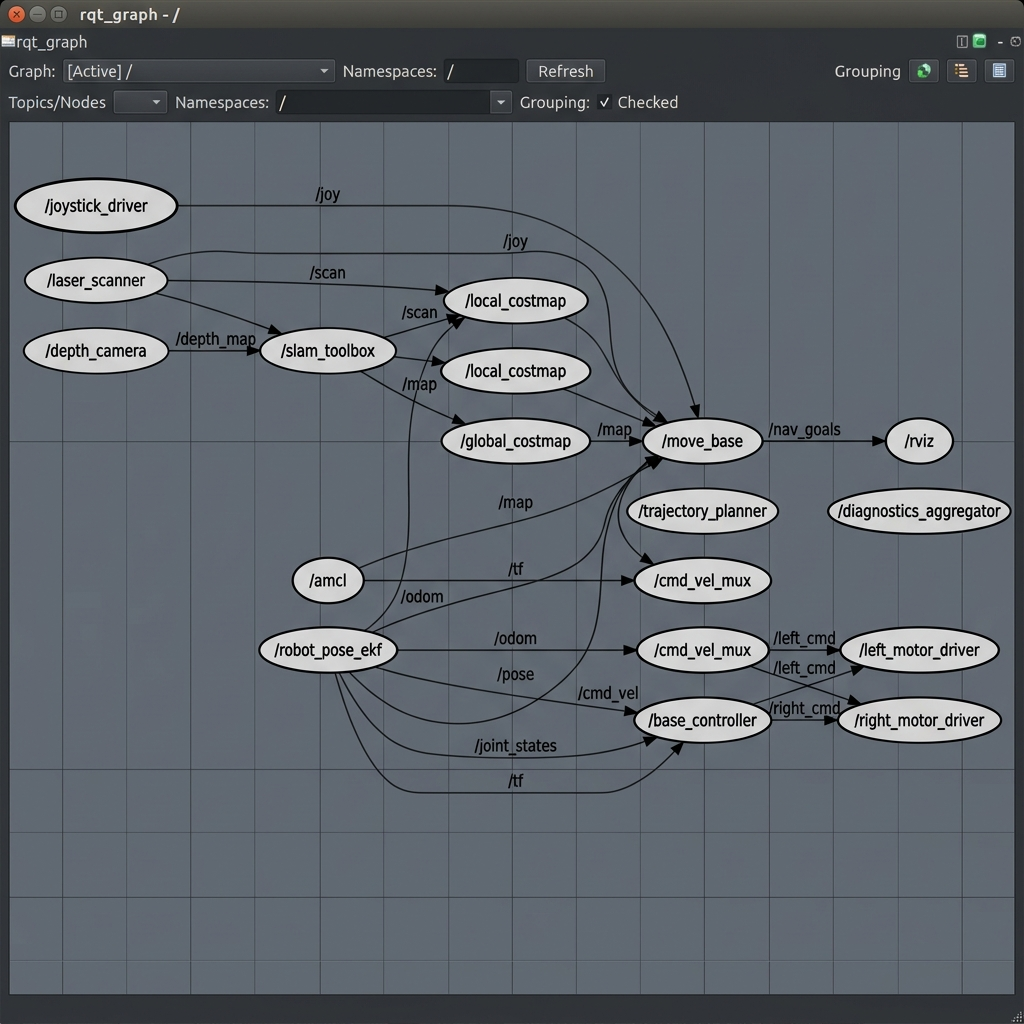
\includegraphics[width=0.83\linewidth,height=0.32\textheight,keepaspectratio]{rqt_graph.png}
\end{frame}

% 7
\begin{frame}{Môi trường mô phỏng Gazebo/Ignition}
\begin{columns}[c]
\column{0.50\textwidth}
\begin{itemize}
  \item Mô phỏng robot, mặt sàn, vật cản, mục tiêu và cảm biến.
  \item Cho phép kiểm thử lặp lại, an toàn, chi phí thấp.
  \item Topic ROS2 giống hệ robot thật, thuận lợi chuyển sang thực nghiệm.
  \item Quan sát song song bằng Gazebo và RViz.
\end{itemize}
\column{0.46\textwidth}\centering\img{1.0}{turtlebot4_gazebo.png}
\end{columns}
\end{frame}

% 8
\begin{frame}{Hệ cảm biến: LiDAR, RGB-D, Odometry, TF}
\begin{tabular}{p{0.24\textwidth} p{0.30\textwidth} p{0.36\textwidth}}
\toprule
\textbf{Thành phần} & \textbf{Dữ liệu} & \textbf{Vai trò}\\
LiDAR & \topic{/scan} & SLAM, tránh vật cản, đo khoảng cách 2D\\
Camera RGB-D & RGB + depth & Phát hiện mục tiêu, tính tọa độ 3D\\
Odometry & \topic{/odom} & Ước lượng chuyển động tương đối\\
TF/TF2 & transform frames & Liên kết \topic{map}, \topic{odom}, \topic{base\_link}, camera\\
\bottomrule
\end{tabular}
\end{frame}

% 9
\begin{frame}{Vai trò LiDAR trong SLAM và tránh vật cản}
\begin{columns}[c]
\column{0.50\textwidth}
\begin{itemize}
  \item Quét khoảng cách quanh robot theo mặt phẳng 2D.
  \item SLAM Toolbox dùng \topic{/scan} để cập nhật occupancy grid.
  \item Nav2 dùng costmap để tránh vật cản khi bám đường.
  \item Chất lượng phụ thuộc TF, nhiễu quét và tốc độ robot.
\end{itemize}
\column{0.46\textwidth}\centering\img{1.0}{laserscan.png}
\end{columns}
\end{frame}

% 10
\begin{frame}{Camera RGB-D + YOLOv8n}
\begin{columns}[c]
\column{0.52\textwidth}
\begin{itemize}
  \item YOLOv8n nhận ảnh RGB, xuất nhãn, độ tin cậy, bounding box.
  \item Ảnh depth cung cấp khoảng cách tại vùng bbox.
  \item Mô hình nhỏ, phù hợp chạy thời gian thực trong mô phỏng.
  \item Kết quả phát hiện được gửi cho Mission Manager.
\end{itemize}
\column{0.42\textwidth}\centering\img{1.0}{yolo_detection.png}
\end{columns}
\end{frame}

% 11
\begin{frame}{Định vị mục tiêu 3D từ bbox + depth}
\begin{columns}[c]
\column{0.50\textwidth}
\begin{itemize}
  \item Lấy tâm bbox: $(u, v)$.
  \item Đọc độ sâu trung vị $Z$ trong vùng bbox để giảm nhiễu.
  \item Chiếu ngược qua nội tại camera:
\end{itemize}
\[
X=\frac{(u-c_x)Z}{f_x}, \qquad Y=\frac{(v-c_y)Z}{f_y}
\]
\begin{itemize}
  \item Dùng TF đổi từ frame camera sang \topic{map}/\topic{odom}.
\end{itemize}
\column{0.42\textwidth}\centering\img{1.0}{yolo_concept.png}
\end{columns}
\end{frame}

% 12
\begin{frame}{SLAM Toolbox: bản đồ và pose robot}
\begin{columns}[c]
\column{0.52\textwidth}
\begin{itemize}
  \item Nhận dữ liệu LiDAR + TF để xây dựng bản đồ 2D.
  \item Cập nhật pose robot trong hệ \topic{map}.
  \item Bản đồ occupancy grid là đầu vào cho Nav2.
  \item Có thể lưu bản đồ để tái sử dụng cho điều hướng.
\end{itemize}
\column{0.42\textwidth}\centering\img{1.0}{map.png}
\end{columns}
\end{frame}

% 13
\begin{frame}{Nav2: goal, lập kế hoạch, /cmd\_vel}
\begin{columns}[c]
\column{0.52\textwidth}
\begin{itemize}
  \item Nhận goal từ RViz, Patrol Node hoặc Mission Manager.
  \item Global planner tạo đường đi trên bản đồ.
  \item Local planner tránh vật cản bằng costmap cục bộ.
  \item Controller sinh \topic{/cmd\_vel} cho robot vi sai.
\end{itemize}
\column{0.42\textwidth}\centering\img{1.0}{rviz_nav2.png}
\end{columns}
\end{frame}

% 14
\begin{frame}{Cơ cấu chấp hành vi sai TurtleBot4}
\begin{columns}[c]
\column{0.50\textwidth}
\begin{itemize}
  \item Hai bánh chủ động trái/phải điều khiển độc lập.
  \item Robot tiến khi hai bánh cùng chiều, quay khi lệch vận tốc.
  \item Lệnh điều khiển: vận tốc tuyến tính $v$ và vận tốc góc $\omega$.
\end{itemize}
\[
  v=\frac{r}{2}(\omega_R+\omega_L),\quad
  \omega=\frac{r}{L}(\omega_R-\omega_L)
\]
\column{0.42\textwidth}\centering\img{1.0}{turtlebot4_lite.png}
\end{columns}
\end{frame}

% 15
\begin{frame}{Mission Manager: Patrol → Detect → Approach → Resume}
\begin{center}
\begin{tikzpicture}[node distance=1.20cm,>=Latex]
\tikzstyle{state}=[draw=ptitred,rounded corners,fill=softred,minimum width=2.05cm,minimum height=0.78cm,align=center,font=\bfseries]
\node[state] (patrol) {Patrol};
\node[state,right=of patrol] (detect) {Detect};
\node[state,right=of detect] (approach) {Approach};
\node[state,right=of approach] (resume) {Resume};
\draw[->,thick,ptitred] (patrol)--node[above,font=\scriptsize]{YOLO hit}(detect);
\draw[->,thick,ptitred] (detect)--node[above,font=\scriptsize]{3D goal}(approach);
\draw[->,thick,ptitred] (approach)--node[above,font=\scriptsize]{done}(resume);
\draw[->,thick,ptitdark,bend left=35] (resume.south) to node[below,font=\scriptsize]{next waypoint} (patrol.south);
\end{tikzpicture}
\end{center}
\begin{itemize}
  \item Điều phối dữ liệu nhận diện, trạng thái Nav2 và danh sách waypoint.
  \item Tính điểm tiếp cận an toàn, không đi thẳng vào mục tiêu.
  \item Khôi phục tuần tra sau khi hoàn tất hành động tiếp cận.
\end{itemize}
\end{frame}

% 16
\begin{frame}{Luồng dữ liệu toàn hệ thống}
\begin{center}
\begin{tikzpicture}[node distance=0.80cm and 0.95cm,>=Latex]
\tikzstyle{box}=[draw=ptitred,rounded corners,fill=softred,minimum width=2.4cm,minimum height=0.72cm,align=center,font=\small\bfseries]
\node[box] (lidar) {LiDAR /scan};
\node[box,below=of lidar] (cam) {RGB-D camera};
\node[box,right=of lidar] (slam) {SLAM Toolbox};
\node[box,right=of cam] (yolo) {YOLOv8n + depth};
\node[box,right=1.55cm of slam] (nav) {Nav2};
\node[box,right=1.55cm of yolo] (mission) {Mission Manager};
\node[box,right=of nav] (cmd) {/cmd\_vel};
\node[box,right=of cmd] (robot) {Diff-drive};
\draw[->,thick,ptitred] (lidar)--(slam); \draw[->,thick,ptitred] (cam)--(yolo);
\draw[->,thick,ptitred] (slam)--node[above,font=\scriptsize]{map/pose}(nav);
\draw[->,thick,ptitred] (yolo)--node[below,font=\scriptsize]{target 3D}(mission);
\draw[->,thick,ptitred] (mission)--node[right,font=\scriptsize]{goal}(nav);
\draw[->,thick,ptitred] (nav)--(cmd); \draw[->,thick,ptitred] (cmd)--(robot);
\draw[->,thick,ptitdark,bend left=28] (robot.north) to node[above,font=\scriptsize]{odom/TF} (slam.north);
\end{tikzpicture}
\end{center}
\end{frame}

% 17
\begin{frame}{Kết quả mô phỏng và topic kiểm tra}
\begin{columns}[c]
\column{0.50\textwidth}
\begin{itemize}
  \item Gazebo khởi tạo TurtleBot4 Lite và môi trường thành công.
  \item RViz hiển thị map, costmap, TF, laser scan, path.
  \item Topic kiểm tra: \topic{/scan}, \topic{/odom}, \topic{/tf}, \topic{/cmd\_vel}.
  \item YOLO phát hiện mục tiêu; Nav2 điều hướng robot theo goal.
\end{itemize}
\column{0.46\textwidth}\centering\img{1.0}{rviz_nav2.png}
\end{columns}
\end{frame}

% 18
\begin{frame}{Kết quả nhận thức mục tiêu}
\begin{columns}[c]
\column{0.50\textwidth}
\begin{itemize}
  \item Bounding box khoanh vùng mục tiêu trong ảnh RGB.
  \item Depth map cung cấp khoảng cách đến vùng phát hiện.
  \item Tọa độ mục tiêu được chuyển sang frame toàn cục bằng TF.
  \item Mission Manager dùng tọa độ này để tạo goal tiếp cận.
\end{itemize}
\column{0.46\textwidth}\centering\img{1.0}{yolo_detection.png}
\end{columns}
\end{frame}

% 19
\begin{frame}{Hạn chế và hướng phát triển}
\begin{columns}[T]
\column{0.48\textwidth}
\begin{block}{Hạn chế}
\begin{itemize}
  \item Kết quả chủ yếu trong mô phỏng.
  \item Cảm biến mô phỏng chưa phản ánh đủ nhiễu thực tế.
  \item YOLO phụ thuộc ánh sáng, góc nhìn và dữ liệu huấn luyện.
\end{itemize}
\end{block}
\column{0.48\textwidth}
\begin{block}{Hướng phát triển}
\begin{itemize}
  \item Triển khai trên TurtleBot4 thật.
  \item Đánh giá định lượng: thời gian, sai số, tỉ lệ phát hiện.
  \item Cải thiện tiếp cận mục tiêu và tránh vật cản động.
\end{itemize}
\end{block}
\end{columns}
\end{frame}

% 20
\begin{frame}{Kết luận}
\begin{itemize}
  \item Hệ thống mô phỏng thể hiện đầy đủ chuỗi cảm biến → xử lý → điều khiển → chấp hành.
  \item LiDAR, RGB-D, SLAM Toolbox, Nav2 và YOLOv8n phối hợp cho nhiệm vụ tự hành.
  \item Mission Manager tạo hành vi cấp cao: tuần tra, phát hiện, tiếp cận, tiếp tục.
  \item Kết quả là nền tảng để mở rộng sang robot thật và môi trường phức tạp hơn.
\end{itemize}
\vspace{0.35cm}
\begin{center}
{\Large\bfseries Cảm ơn thầy và các bạn đã lắng nghe!}
\end{center}
\end{frame}

\end{document}



